%-----------------------------------------------------------------------------------------
\clearpage
\section{Project Plan and Time Management}
%-----------------------------------------------------------------------------------------
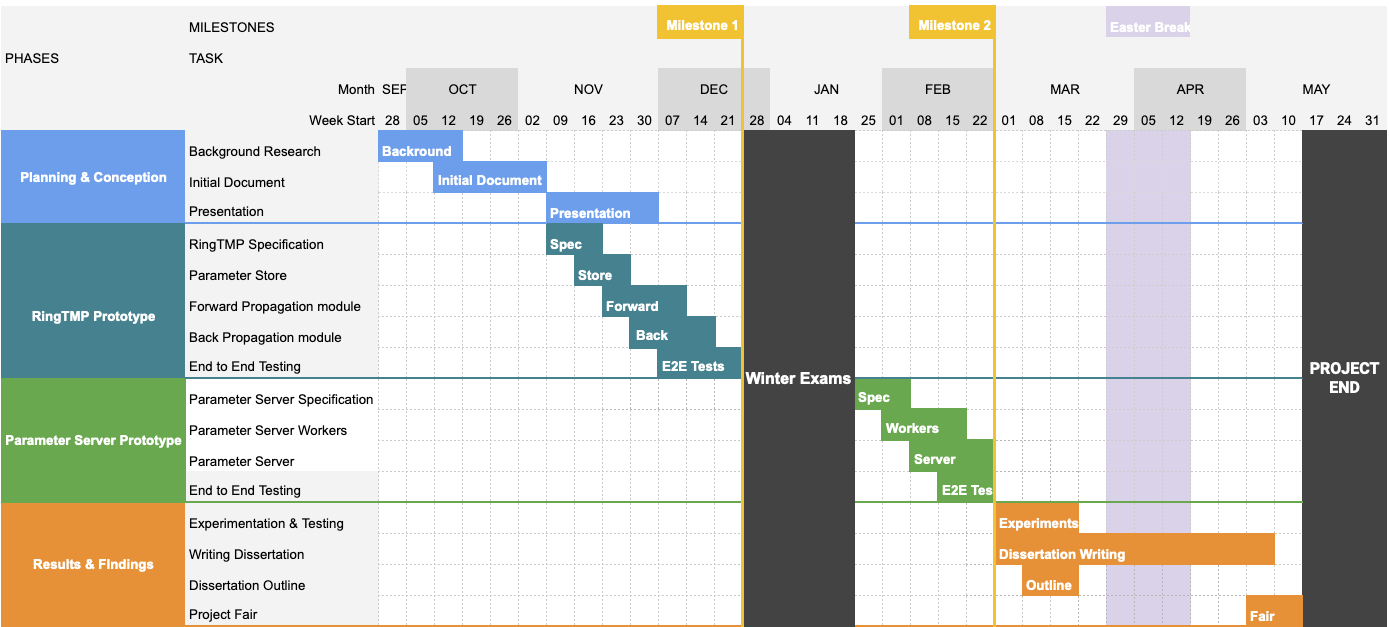
\includegraphics[width=16cm, height=8cm]{BetterGant.png}

The gant chart above outlines the order and time frame each task should take in
order complete this dissertation on time and to a high quality. After
researching the background and submitting the initial document. Building a
RingTMP prototype of my system is the most important task to embark on. It is
better to do this first as it will take the longest time to produce and has the
most 'unknown unknowns', moreover this is the centrepiece of my project if I
have not finished this there will be no dissertation to write. I then take a
month break to revise for my exams. I acknowledge that this is a long time,
however semester 1 modules contribute more to my final grade than my
dissertation does, therefore its important this project isn't detrimental to my
grades in other modules. After Christmas I'll start work on a basic prototype of
a parameter server. This will use the same tools and languages as my framework.
In this way it will be easy to compare and contrast the benefits and
shortcomings of each system on a level playing field. Once Both pieces of
software have been complete I will run various tests to see how well my aims
have been achieved. While I'm conducting these tests I shall also be writing up
my results. Once my experiments have finished I shall start working on my
dissertation document in earnest. I'll hand in my outline a week before easter
break and shall keep working till it is complete, hopefully sometime before the
project deadline (TBC) sometime in May.

\subsection{Applied Methodology}

My project lends itself to using an experimental research methodology to collect
my findings, with this in mind is paramount to ensure that my results are taken
is as controlled conditions as possible. I will achieve this by
creating two software prototypes, one is my new novel machine learning
framework, the other is the established parameter server design. I will make
these using the same languages and tools as each other. Only the architecture
will differ, meaning comparisons of the two systems will only reflect the
performance of the respective architectures. On these systems I will conduct a
series of tests. Each of these tests will compare each system to one another and
will correspond to the aims I outlined in the introduction:
\begin{itemize}
    \item To compare the efficiency of the systems we can measure the idle time
    of each worker in each of the systems and divide that by the time each
    system took to train a model on some basic task. This will give us a
    percentage of how much time the machine spend processing and how much time
    was spent on communication between nodes. This same experiment can be
    repeated with a different amount of nodes to see how the results change.
    \item To compare the progress made per iteration, the loss function can be
    measured for each iteration on both of the systems, then it is trivial to
    see which ones makes the most progress.
    \item To measure scalability both systems can be run with a varying number
    of different nodes. In all experiments they are given the same dataset to be
    trained on. We can measure how long it takes for them to complete the task,
    and how well both systems scale when more nodes are added.
    \item To measure resilience a node can be permanently or temporarily removed
    from each system while a model is being trained. Then the success of its
    mitigation and recovery strategies can be assessed.
    \item To discover the limits of how large a Neural Network each system can
    hold. Tests which incrementally increase the amount of layers and number of
    layers until the system crashes can be run.
\end{itemize}
By doing all this I can measure the performance between these two systems and
accurately assess my architecture's performance relative to the parameter server.

\subsection{Risk Assessment}

A dissertation is a long arduous process in which many things could go wrong.
Hence it is best to identify possible hazards and decide how to mitigate them
before they happen.



    
% \begin{tabular}{|c|c|c|c|}
% \hline
% Risk & Likelihood & Potential & Mitigation \\
% & & Impact  & \\
% \hline
% Completed & The requirement is implemented or fulfilled \\
% \hline
% Partial & The requirement is partially implemented or fulfilled \\
% Not Completed & The requirement is not implemented or fulfilled \\
% FR & Functional Requirement \\
% NFR & Non Functional Requirement \\
% FS & Functional Specification \\
% NFS & Non Functional Specification\\
% \end{tabular}

% \begin{table}[]
%     \begin{tabular}{|l|l|l|l|l|}
%     \hline
%     a & \begin{tabular}[c]{@{}l@{}}Hello there\\ henuy\end{tabular} & \begin{tabular}[c]{@{}l@{}}what yo \\ doing\end{tabular} & c & v \\ \hline
%       &                                                             &                                                          &   &   \\ \hline
%       &                                                             &                                                          &   &   \\ \hline
%       &                                                             &                                                          &   &   \\ \hline
%     \end{tabular}
% \end{table}

% \begin{tabular}{|c|c|c|}
% \hline
% Risk & Likelihood & Potential Impact & Mitigation \\
% \hline
% I die & Low & I cannot complete dissertation & N/A \\
% \end{tabular}